\documentclass[10pt,a4paper]{article}
\usepackage{fontspec}
\usepackage[slantfont, boldfont]{xeCJK}
\usepackage{graphicx}

\XeTeXlinebreaklocale "zh"
\XeTeXlinebreakskip = 0pt plus 1pt minus 0.1pt

\setCJKmainfont{Adobe Heiti Std}
\parindent 2em

\begin{document}
\title{Voici图像处理软件的界面改进}
\author{宋文灏}
\date{\today}
\maketitle
\section{工具栏的图标}
为工具栏的按钮增加了图标,这让他们更容易辨认。\\

改进前:\\
\indent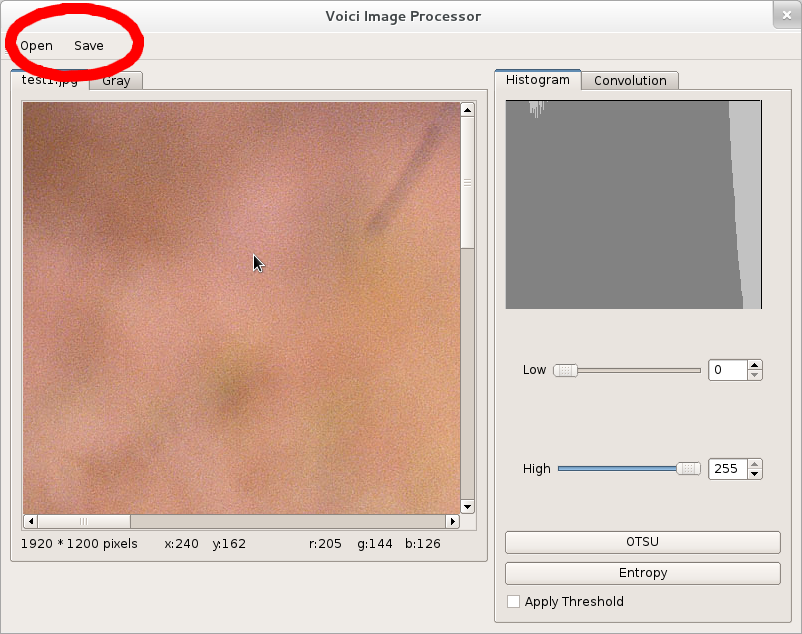
\includegraphics[width=0.65\textwidth]{icon_origin.png}\\

改进后:\\
\indent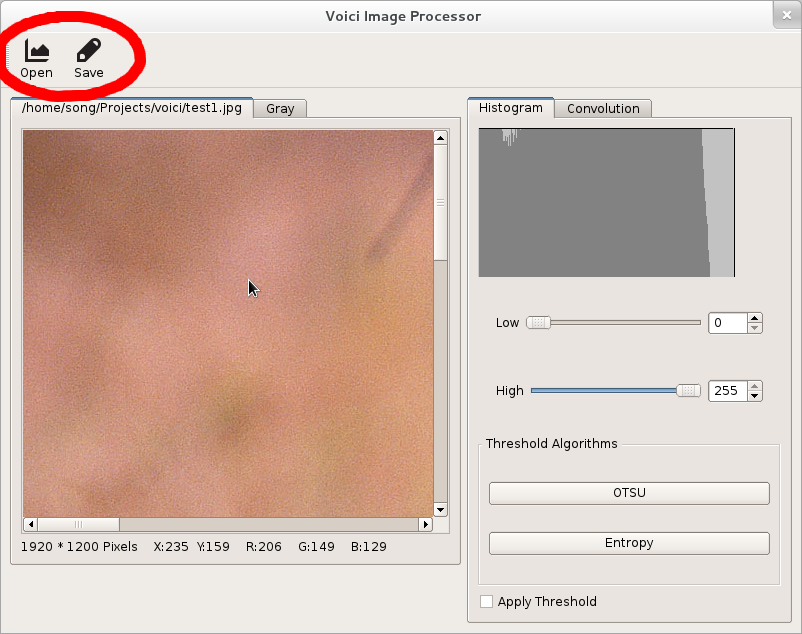
\includegraphics[width=0.65\textwidth]{icon_improved.png}

\pagebreak


\section{分组}
把有类似功能的按钮分在一组,将不同的功能分开,使用户能够更好地识别和使用。\\

改进前:\\
\indent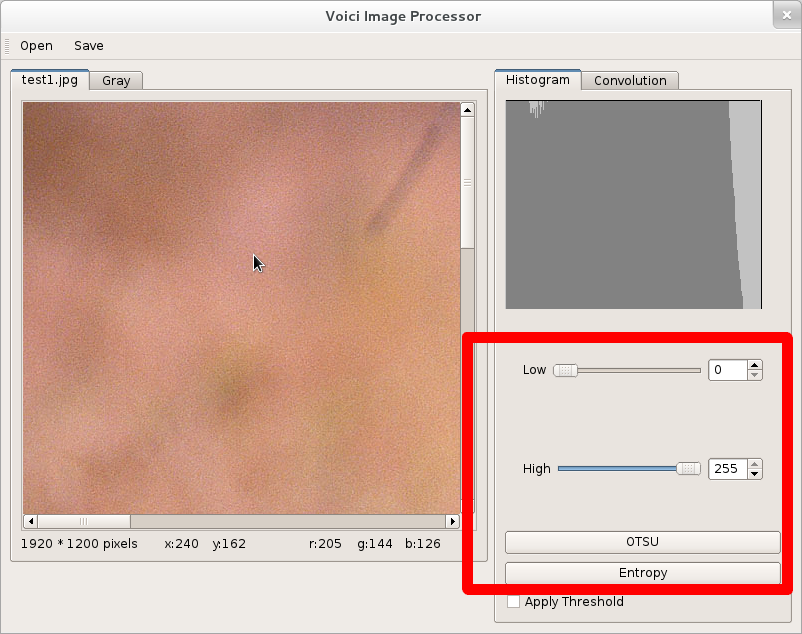
\includegraphics[width=0.65\textwidth]{group_origin.png}\\

改进后:\\
\indent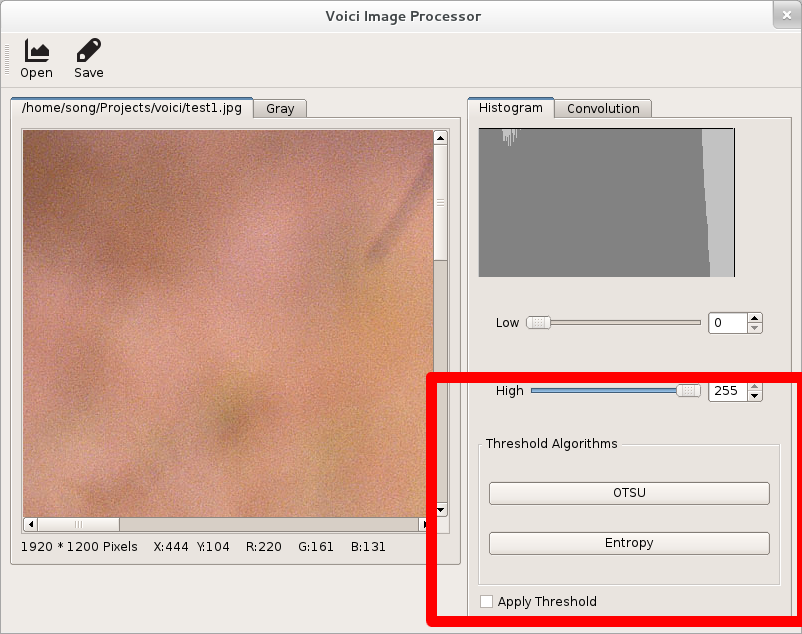
\includegraphics[width=0.65\textwidth]{group_improved.png}

\pagebreak

\section{算子中间项的颜色}
改变算子中间项的颜色,相比与下方的数字,给用户一个更直观的信息。\\

改进前:\\
\indent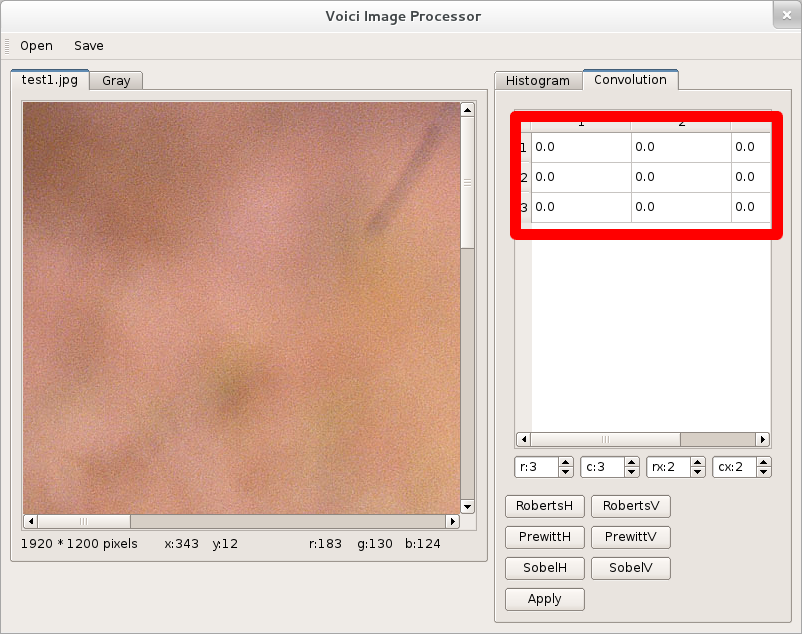
\includegraphics[width=0.65\textwidth]{item_origin.png}\\

改进后:\\
\indent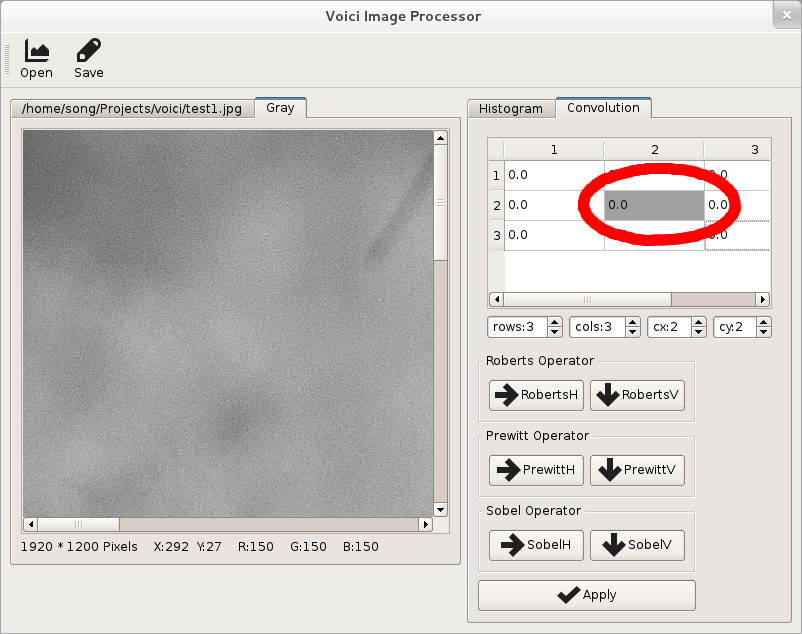
\includegraphics[width=0.65\textwidth]{item_improved.png}

\pagebreak

\section{按键组}
把一类的按钮放在一组。在同一组内,同时使用图标来加强按钮功能的细微差别。\\

改进前:\\
\indent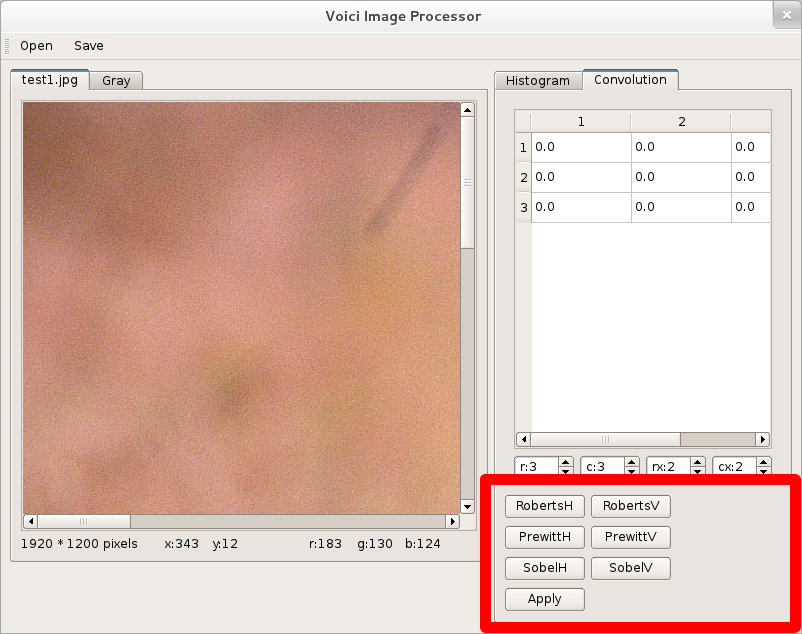
\includegraphics[width=0.65\textwidth]{icon_and_group_origin.png}\\

改进后:\\
\indent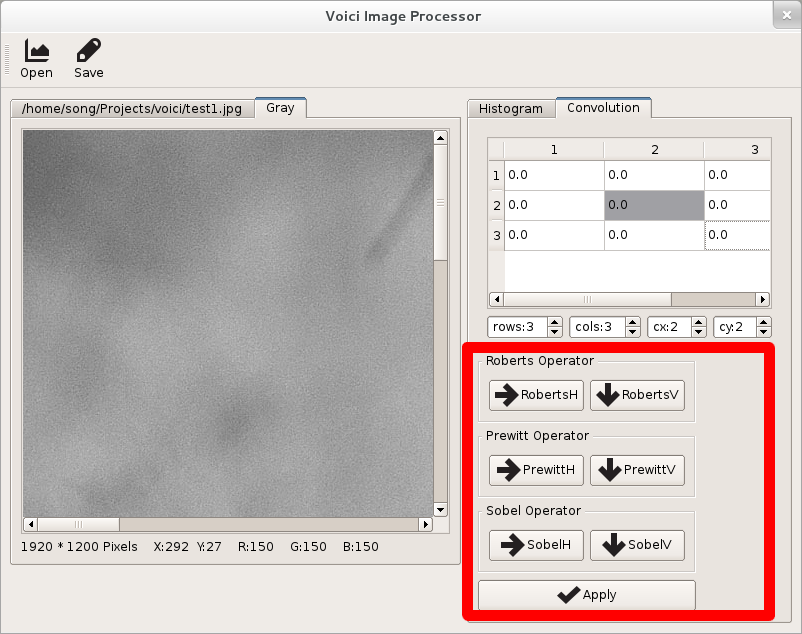
\includegraphics[width=0.65\textwidth]{icon_and_group_improved.png}

\pagebreak

\section{鼠标图形}
在改进的版本中,当鼠标移动到图片区域那时,鼠标的图形会变成十字。

由于我使用的截图软件不会在截图中体现鼠标的区别,你可以自己运行程序尝试一下。

\section{国际化}
在英文版的基础上,做了中文版。这使得软件更容易被不同语言的使用者理解。\\

改进后:\\
\indent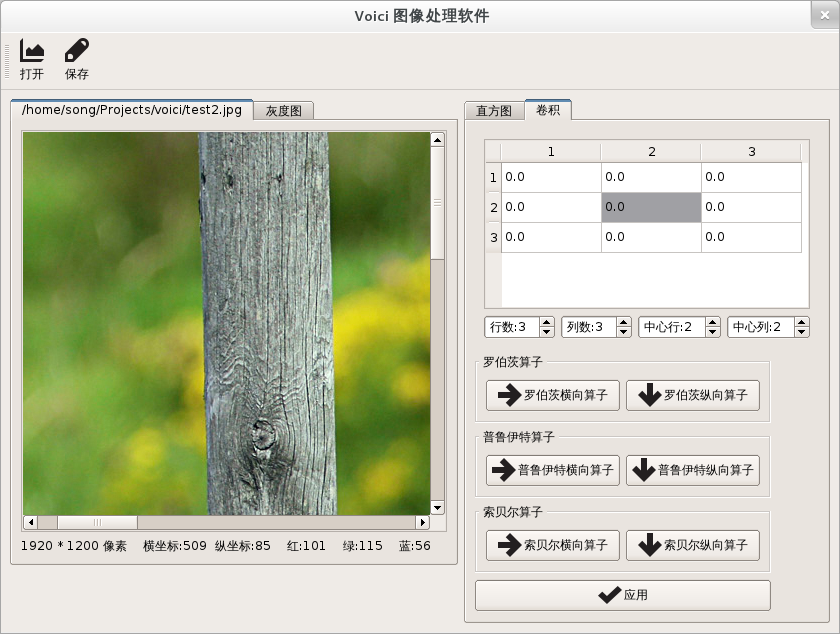
\includegraphics[width=0.65\textwidth]{chinese_improved.png}

\section{为什么没有改变界面的整体颜色}
我觉得默认的颜色足够好了。尽管它不是很酷,但是用户在使用一段时间后,不会感到眼睛不适。我认为实用是更重要的因素。

\end{document}


